\documentclass{fizykalab}

% Ustawienia do tabelki

\wydzial{WI}
\autorjeden{Dawid Komęza}
\autordwa{Magdalena Śmietana}
\rok{II}
\grupa{14}
\zespol{2}
\temat{Halotron}
\nrcwiczenia{43}
\datawykonania{24.10.2025}
\dataoddaniajeden{07.11.2025}
\zwrotdopoprawy{}
\dataoddaniadwa{}
\datazaliczenia{}

\begin{document}

\maketitle

\section{Cel ćwiczenia}
Celem ćwiczenia jest cechowanie halotronu przy użyciu pola magnetycznego o znanej indukcji, a także pomiar przestrzennego rozkładu pola cewki kołowej i magnesu ferrytowego.

\section{Wstęp teoretyczny i wzory}

\subsection{Pole elektryczne i natężenie pola elektrycznego}
Wektor natężenia pola elektrycznego $\mathbf{E}$ definiujemy jako siłę działającą na jednostkowy ładunek dodatni:
\begin{equation}
    \mathbf{E} = \frac{\mathbf{F}}{q}
\end{equation}

\subsection{Potencjał i napięcie}
Napięcie elektryczne $U$ między dwoma punktami A i B to różnica potencjałów:
\begin{equation}
    U_{AB} = V_A - V_B
\end{equation}

Praca wykonana przez pole elektryczne przy przenoszeniu ładunku $q$:
\begin{equation}
    W = qU_{AB} = q\int_A^B \mathbf{E} \cdot d\mathbf{l}
\end{equation}

\subsection{Prawo Ohma}
Wersja makroskopowa:
\begin{equation}
    U = IR
\end{equation}

Wersja mikroskopowa:
\begin{equation}
    \mathbf{j} = \sigma \mathbf{E}
\end{equation}
gdzie $\sigma$ jest przewodnością elektryczną, a $\mathbf{j}$ gęstością prądu.

\subsection{Gęstość prądu, prędkość unoszenia i koncentracja nośników}
Gęstość prądu: $\mathbf{j} = \frac{I}{S}$, prędkość unoszenia $\mathbf{v}$ to średnia prędkość nośników, koncentracja $n$ to liczba nośników w jednostce objętości. Związek między nimi:
\begin{equation}
    \mathbf{j} = nq\mathbf{v}
\end{equation}

\subsection{Pole magnetyczne}
Indukcja magnetyczna $\mathbf{B}$ charakteryzuje pole magnetyczne (jednostka: tesla [T]).

Linie pola wokół prostoliniowego przewodnika tworzą okręgi koncentryczne (kierunek: reguła prawej dłoni). Dla cewki linie są równoległe do osi wewnątrz i zamykają się na zewnątrz.

\subsection{Prawo Biota-Savarta}
\begin{equation}
    d\mathbf{B} = \frac{\mu_0}{4\pi} \frac{I d\mathbf{l} \times \mathbf{r}}{r^3}
\end{equation}

Dla przewodnika kołowego o promieniu $R$ indukcja w środku:
\begin{equation}
    B = \frac{\mu_0 I}{2R}
\end{equation}

Dla cewki z $N$ zwojami:
\begin{equation}
    B_0 = \frac{\mu_0 N I}{2R}
\end{equation}

\subsection{Siła Lorentza}
\begin{equation}
    \mathbf{F} = q(\mathbf{E} + \mathbf{v} \times \mathbf{B})
\end{equation}

W jednorodnym polu magnetycznym ładunek poruszający się prostopadle do $\mathbf{B}$ wykonuje ruch po okręgu o promieniu:
\begin{equation}
    r = \frac{mv}{qB}
\end{equation}

Przy składowej prędkości równoległej do $\mathbf{B}$ tor jest spiralny.

\subsection{Zjawisko Halla}

\begin{figure}[h]
\centering
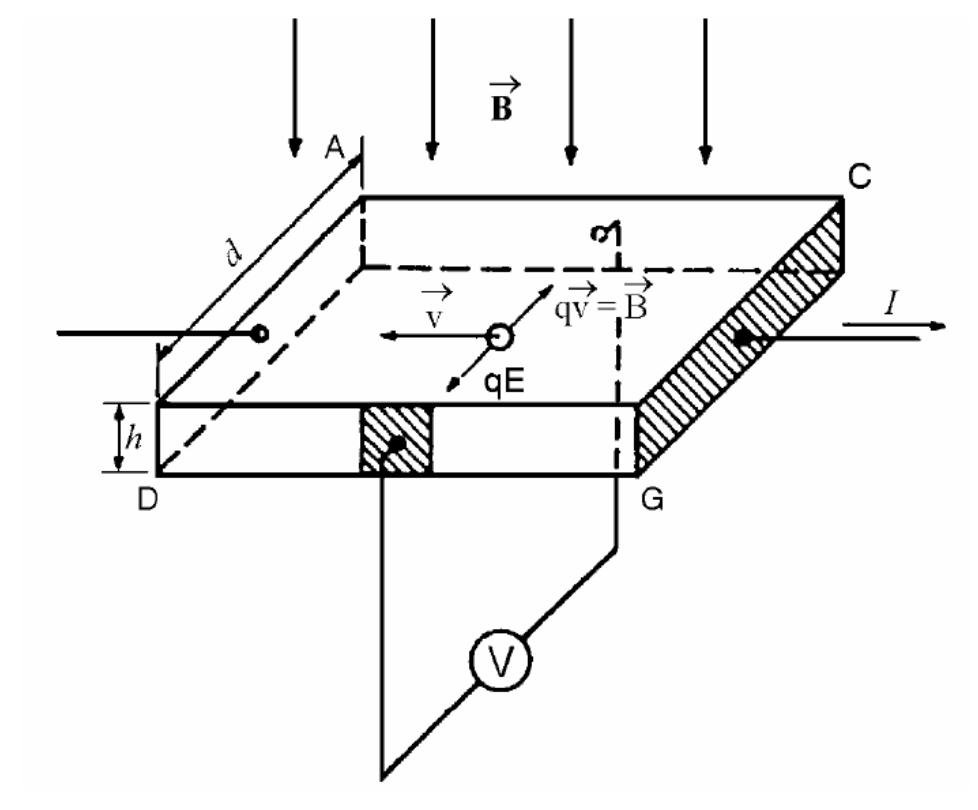
\includegraphics[width=0.6\textwidth]{halotron.png}
\caption{Schematyczne przedstawienie zasady działania halotronu}
\label{fig:halotron}
\end{figure}

Napięciem Halla nazywamy różnicę potencjałów powstającą w przewodniku z prądem umieszczonym w polu magnetycznym. Na elektrony w halotronie działa siła Lorentza:
\begin{equation}
    \mathbf{F} = q\mathbf{v} \times \mathbf{B}
\end{equation}

Dla napięcia Halla $U_H$ występuje pole elektryczne $E_H = \frac{U_H}{d}$. Na elektrony działa więc siła:
\begin{equation}
    F_E = q \cdot E_H
\end{equation}

Obie te siły działają w przeciwnych kierunkach i w stanie równowagi otrzymujemy:
\begin{equation}
    U_H = vBd
    \label{eq:uh1}
\end{equation}

Gęstość prądu wyrażamy jako $j = \frac{I}{dh}$, a przyjmując $n$ jako koncentrację nośników (liczba nośników prądu w jednostce objętości), mamy:
\begin{equation}
    j = vnq
    \label{eq:j}
\end{equation}

Łącząc równania~\eqref{eq:uh1} i~\eqref{eq:j} otrzymujemy:
\begin{equation}
    U_H = \frac{1}{nqh}IB
    \label{eq:uh2}
\end{equation}

Współczynnik proporcjonalności $c = \frac{1}{nqh}$ to stała halotronu.

W efekcie oporu warstwy półprzewodnika zastosowanego do budowy halotronu powstaje dodatkowe napięcie $U_R$ proporcjonalne do prądu halotronu. Mierzone napięcie wynosi więc:
\begin{equation}
    U = U_H + U_R = cIB + RI
    \label{eq:utotal}
\end{equation}

\subsection{Indukcja na osi cewki}
Natężenie pola magnetycznego na osi cewki kołowej liczymy korzystając z prawa Biota-Savarta. Wynosi ono:
\begin{equation}
    B_0 = \frac{\mu_0 N I_s}{2R}
    \label{eq:b0}
\end{equation}

Wykonując pomiary na osi solenoidu w odległości $z$ od jego środka otrzymujemy następujący wzór na indukcję magnetyczną:
\begin{equation}
    B(z) = \frac{B_0}{\left(1 + \frac{z^2}{R^2}\right)^{3/2}}
    \label{eq:bz}
\end{equation}

\section{Aparatura pomiarowa}
\begin{figure}[h!]
\centering
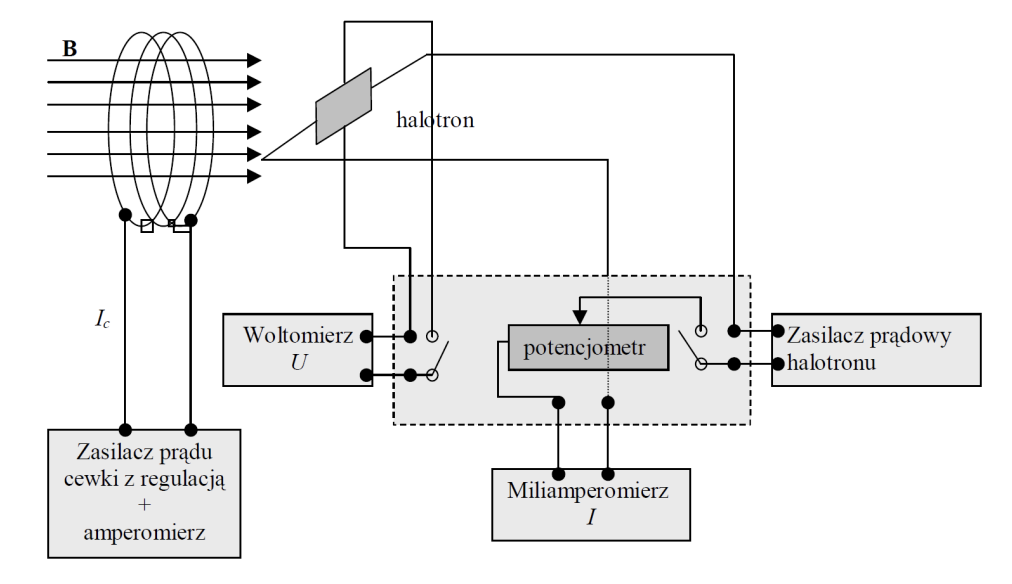
\includegraphics[width=0.6\textwidth]{halotron_uklad.png}
\caption{Schemat układu pomiarowego halotronu}
\label{fig:halotron_uklad}
\end{figure}

W skład układu pomiarowego weszły następujące elementy:
\begin{enumerate}
    \item Halotron wraz z zasilaczem oraz podłączonymi miliamperomierzem i woltomierzem, a także potencjometrem regulującym natężenie prądu.
    \item Cewka z zasilaczem, regulacją prądu oraz amperomierzem.
\end{enumerate}


\section{Wnioski}

\end{document}
